\documentclass[12pt]{article}
%%%%%%%%%%%%%%%%
% Packages
%%%%%%%%%%%%%%%%

\usepackage[top=1cm,bottom=1.25cm,left=1.25cm,right= 1.25cm]{geometry}
\usepackage[parfill]{parskip}
\usepackage{graphicx, fontspec, xcolor,multicol, enumitem, setspace, amsmath, changepage}
\DeclareGraphicsRule{.tif}{png}{.png}{`convert #1 `dirname #1`/`basename #1 .tif`.png}

%%%%%%%%%%%%%%%%
% User defined colors
%%%%%%%%%%%%%%%%

% Pantone 2015 Fall colors
% http://iwork3.us/2015/02/18/pantone-2015-fall-fashion-report/
% update each semester or year

\xdefinecolor{custom_blue}{rgb}{0, 0.32, 0.48} % FROM SPRING 2016 COLOR PREVIEW
\xdefinecolor{custom_darkBlue}{rgb}{0.20, 0.20, 0.39} % Reflecting Pond  
\xdefinecolor{custom_orange}{rgb}{0.96, 0.57, 0.42} % Cadmium Orange
\xdefinecolor{custom_green}{rgb}{0, 0.47, 0.52} % Biscay Bay
\xdefinecolor{custom_red}{rgb}{0.58, 0.32, 0.32} % Marsala

\xdefinecolor{custom_lightGray}{rgb}{0.78, 0.80, 0.80} % Glacier Gray
\xdefinecolor{custom_darkGray}{rgb}{0.35, 0.39, 0.43} % Stormy Weather

%%%%%%%%%%%%%%%%
% Color text commands
%%%%%%%%%%%%%%%%

%orange
\newcommand{\orange}[1]{\textit{\textcolor{custom_orange}{#1}}}

% yellow
\newcommand{\yellow}[1]{\textit{\textcolor{yellow}{#1}}}

% blue
\newcommand{\blue}[1]{\textit{\textcolor{blue}{#1}}}

% green
\newcommand{\green}[1]{\textit{\textcolor{custom_green}{#1}}}

% red
\newcommand{\red}[1]{\textit{\textcolor{custom_red}{#1}}}

%%%%%%%%%%%%%%%%
% Coloring titles, links, etc.
%%%%%%%%%%%%%%%%

\usepackage{titlesec}
\titleformat{\section}
{\color{custom_blue}\normalfont\Large\bfseries}
{\color{custom_blue}\thesection}{1em}{}
\titleformat{\subsection}
{\color{custom_blue}\normalfont}
{\color{custom_blue}\thesubsection}{1em}{}

\newcommand{\ttl}[1]{ \textsc{{\LARGE \textbf{{\color{custom_blue} #1} } }}}

\newcommand{\tl}[1]{ \textsc{{\large \textbf{{\color{custom_blue} #1} } }}}

\usepackage[colorlinks=false,pdfborder={0 0 0},urlcolor= custom_orange,colorlinks=true,linkcolor= custom_orange, citecolor= custom_orange,backref=true]{hyperref}

%%%%%%%%%%%%%%%%
% Instructions box
%%%%%%%%%%%%%%%%

\newcommand{\inst}[1]{
\colorbox{custom_blue!20!white!50}{\parbox{\textwidth}{
	\vskip10pt
	\leftskip10pt \rightskip10pt
	#1
	\vskip10pt
}}
\vskip10pt
}

%%%%%%%%%%%
% App Ex number    %
%%%%%%%%%%%

% DON'T FORGET TO UPDATE

\newcommand{\appno}[1]
{2.2}

%%%%%%%%%%%%%%
% Turn on/off solutions       %
%%%%%%%%%%%%%%

% Off
\newcommand{\soln}[2]{$\:$\\ \vspace{#1}}{}

%%% On
%\newcommand{\soln}[2]{\textit{\textcolor{custom_red}{#2}}}{}

%%%%%%%%%%%%%%%%
% Document
%%%%%%%%%%%%%%%%

\begin{document}
\fontspec[Ligatures=TeX]{Helvetica Neue Light}

Dr. \c{C}etinkaya-Rundel \hfill Sta 101: Data Analysis and Statistical Inference \\
Duke University - Department of Statistical Science \hfill \\

\ttl{Application exercise \appno{}: \\
Bayesian inference for drug testing}

\inst{$\:$ \\
Team name: \rule{10cm}{0.5pt} \\
$\:$ \\
Lab section: $\qquad$ 8:30 $\qquad$ 10:05 $\qquad$ 11:45 $\qquad$ 1:25 $\qquad$ 3:05 $\qquad$ 4:40 \\
$\:$ \\
Write your responses in the spaces provided below. WRITE LEGIBLY and SHOW ALL WORK! 
Only one submission per team is required. One team will be randomly selected and their 
responses will be discussed and graded. Concise and coherent are best!}

Most companies drug test their employees before they start employment, and sometimes regularly during their employment as well. Suppose that a drug test for an illegal drugs is 97\% accurate in the case of a user of that drug, and 92\% accurate in the case of a non-user for that drug. Suppose also that 5\% of the entire population uses that drug.

Show all your work when answering the questions below.

\begin{enumerate}

\item You are the hiring manager at a company that drug tests their employees. You have recently decided to hire a new employee. What is the prior probability that this employee is a user of this drug? (You may assume that this prospective employee is a randomly drawn person from the population.)

\soln{1cm}{P(drug user) = 0.05}

\item The prospective employee gets drug tested, and the test comes out to be positive. What is the probability that they are actually a user for the drug? What is this probability called? Sketch a probability tree for this question.

\soln{6cm}{P(drug user $|$ +) $\rightarrow$ posterior probability\\
\begin{minipage}[c]{0.7\textwidth}
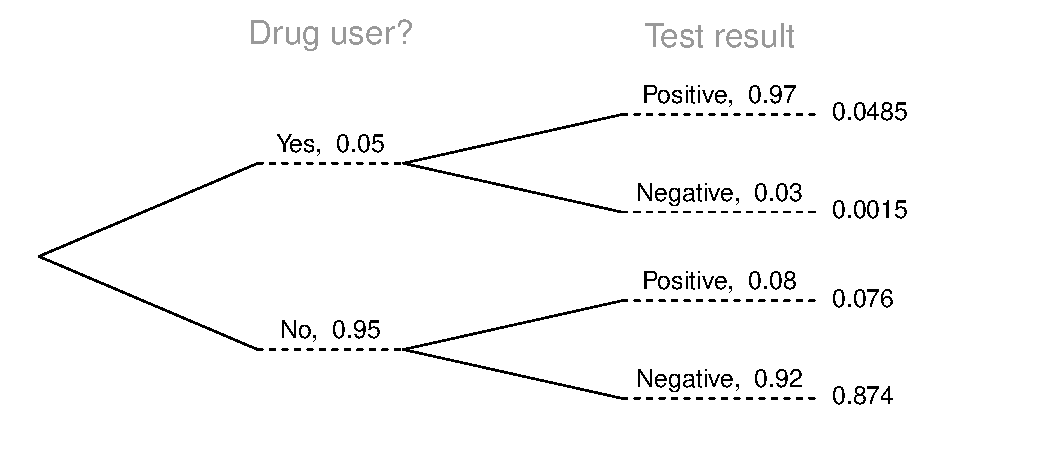
\includegraphics[width = \textwidth]{figures/test1.pdf}
\end{minipage}
\begin{minipage}[c]{0.3\textwidth}
\begin{align*}
&P(drug~user~|~+) \\
&= \frac{P(drug~user~AND~+)}{P(+)} \\
&= \frac{0.0485}{0.0485 + 0.076} \\
&\approx 0.39
\end{align*}
\end{minipage}
}

\item When the employee finds out that they tested positive, they refuse the test results, and say they would like to be tested again. What is the new prior probability you should use for this employee being a user of this drug?

\soln{1cm}{P(drug user) = 0.39}

\item The employee tests positive again in the second test. Should the new probability of them actually being a user of this drug be higher or lower than what you calculated before, or the same? Answer this question before you actually complete the calculations.

\soln{1cm}{Higher.}

\item Finally, calculate the new updated probability that this employee is a user of this drug. When answering this question sketch a probability tree, take a picture, and upload to Sakai as an attachment.

\soln{6cm}{P(drug user $|$ +) $\rightarrow$ posterior probability\\
\begin{minipage}[c]{0.7\textwidth}
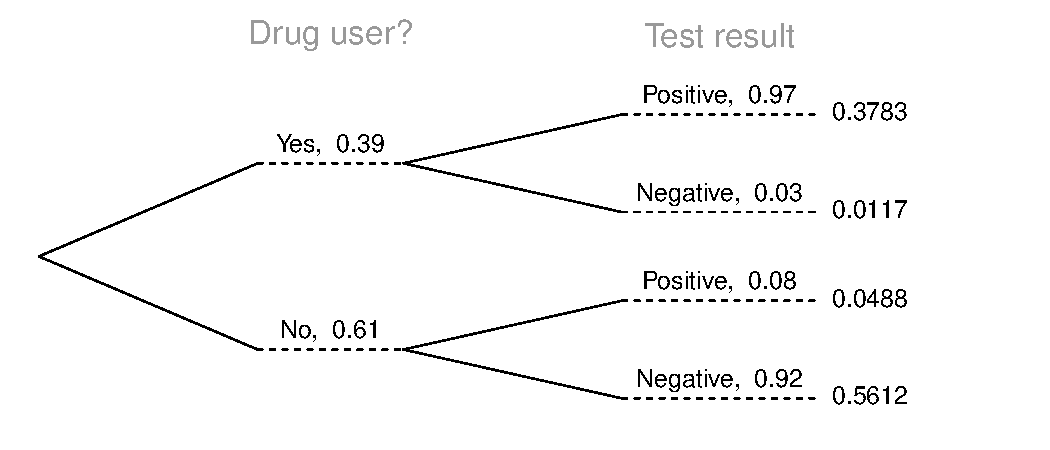
\includegraphics[width = \textwidth]{figures/test2.pdf}
\end{minipage}
\begin{minipage}[c]{0.3\textwidth}
\begin{align*}
&P(drug~user~|~+) \\
&= \frac{P(drug~user~AND~+)}{P(+)} \\
&= \frac{0.3783}{0.3783 + 0.0488} \\
&\approx 0.89
\end{align*}
\end{minipage}
}

\item Based on these results, would you hire this employee? Why or why not?

\soln{1cm}{No, quite likely that the employee is a drug user.}

\end{enumerate}

\end{document}